\documentclass[crop,tikz]{standalone}
\usetikzlibrary{%
    arrows,
    arrows.meta,
    backgrounds,
    calc,
    decorations.pathreplacing,
    fit,
    matrix,
    positioning,
    scopes,
    shadows
}
\usepackage[charter]{mathdesign}

\begin{document}
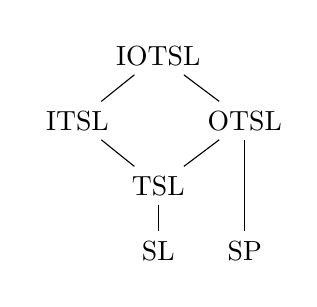
\begin{tikzpicture}
    \matrix (h)  [matrix of nodes, ampersand replacement=\&,
                  column sep=-.4em, row sep=1em,
                 ] {
          \& IOTSL \\
     ITSL \&          \& OTSL \& \\
          \& TSL\\
          \& SL       \& SP\\
    };

    \foreach \Source/\Target in {%
        1-2/2-1,
        1-2/2-3,
        2-1/3-2,
        2-3/3-2,
        3-2/4-2,
        2-3/4-3%
        }
        \draw (h-\Source) to (h-\Target);
\end{tikzpicture}
\end{document}
